\pagebreak
\section{Case study: introducing the Mockingjay attack}

After our review of process injection techniques used by malware groups, we now ask how a CISO in an organisation can stay ahead of the curve,
have a realistic understanding of the threats their organisation might face and develop a resilient cyber-security infrastructure.

Our hypothetical CISO has been active in putting in place an XDR system. This has reduced the manual processes his group needs to
perform --- such as patching individual cybersecurity applications and running separate disjoint processes --- and has leveraged the
vendor's expertise to configure the monitoring of data produced across end-points, servers, cloud networks and
security information and event management (SEIM) systems.

Our enlightened CISO has empowered his team to research ways to improve cyber-security and looks forward to using their
insights to engage with senior stakeholders within the organisation.  He champions his team's achievements and regularly
briefs the board on improvements to understanding their operational risks and mitigation plans.

One of the team's security engineers has come across a new potential exploit and has produced the following case study for the CISO
and his team.  The Mockingjay attack \autocite{Peixoto:2023} is a real and novel process injection attack created by Security Joes, a
``multi-layered MDR \& incident response company'' based in Tel Aviv.  The Security Joes report is an opportunity to assess the organisation's
defence to process injection attacks and how it would respond to such an attack if successful.

\subsection{Introduction}

\textbf{Problem Statement}:

\begin{enumerate}
\item Security Joes has identified a new process injection attack.  The exploit circumvents the allocation
  and permission APIs that most EDR systems monitor.  It  does this by using existing RWX code sections without invoking
  new threads.
\item We may be vulnerable to this attack which could allow a Windows executable to use self-injection or remote injection to deliver a malware payload into our systems.
\item Recently Citrix has reported vulnerabilities in their NetScaler Application Delivery Controller (ADC) and Gateway products that
  could allow:
  \begin{itemize}
  \item \citetitle{CVE-2023-3467} \autocite{CVE-2023-3467}.
  \item \citetitle{CVE-2023-3519} \autocite{CVE-2023-3519}.
  \item \citetitle{CVE-2023-4966} \autocite{CVE-2023-4966}.
  \end{itemize}
\item The Cybersecurity and Infrastructure Security Agency (CISA) has reported that the malware group LockBit \autocite{CISA:2023a} has
  been found to be actively exploiting CVE-2023-4966 and was able to obtain initial access to systems at Boeing Distribution Inc. \autocite{CISA:2023b}.
\end{enumerate}

Our organisation should be prepared for similar attacks, and we should review our cyber-defences in light of this information.
As always, we should seek to prevent any successful attack, but also improve our cyber-resilience in the face of a successful breach.

This case study will:
\begin{enumerate}
\item Review the salient points of the new attack vector, how it may evade our XDR system and how we may identify an attack.
\item Understand ransomware threat actors such as LockBit and how we can detect and respond to a ransomware group's incursion.
\item Prepare a set of recommendations in line with our Cyber-Security Framework (CSF) \autocite{NIST:2018}.
\end{enumerate}


%\subsection{Real-world examples of malware employing process injection on Windows}
\subsection{Detailed analysis of the new process injection method}

Attackers could exploit the Mockingjay technique to circumvent EDR/XDR monitoring and anti-virus software by avoiding
common system API calls used by malware.

It does this by searching for Windows DLLs with a default RWX memory section that can be exploited to run a malware payload.
This is similar to the Nirvana callback code injection that uses NtWriteVirtualMemory and NtProtectVirtualMemory calls, which are
monitored by EDR/XDRs,  but this method avoids those calls.

The DLL and executable exploited in the report were msys-2.0.dll and the GNU ssh.exe, which come part of Visual Studio Community.
The security report was able to demonstrate:

\begin{enumerate}
\item Self-injection: build an executable that directly loads the identified DLL, then inject and then execute the payload. 
\item Remote process injection: create a child process, ssh.exe, that uses loads identified the DLL, then inject a shellcode to initiate
  a remote attack which allowed a back-connect shell session to be opened from a remote system.
\end{enumerate}

An interesting point to note is that the attack code can programmatically construct OS syscall wrappers at run-time without relying
on hard coded definitions or OS data structures.
These call stubs are unmonitored, but they need to be built from a clean and unhooked copy of NTDLL.DLL.
The method is described in the ``Hell's Gate'' article \autocite{smellyvx:2021}.
The significance of this is that the functions within the NTDLL.dll module are wrappers around OS service requests that
the malware payload can exploit. 

Also, payloads are executed without the creation of a new thread, making the detection of this attack by end-point defences harder.


\subsection{Current mitigants}

The first line of our defence of an attack based on the Mockingjay process injection technique will be our XDR system to:
\begin{itemize}
\item Consolidation and preparation phase: detect the code injection attack.
\item Target impact phase: detect the actions of the payload execution, which will be determined by the attacker's motives.
\end{itemize}

Using ``Lifecycle of a Ransomware Incident'' produced by \autocite{Certnz:2021} and the modus-operandi of the LockBit
group \autocite{CISA:2023}, we should anticipate:

\begin{enumerate}
\item Direct attack through our application gateway (Internet-exposed Service).
\item Phishing attack through email.
\end{enumerate}

If either of these two approaches are successful, ransomware groups such as LockBit will use the exploit to:

\begin{enumerate}
\item Exfiltrate data.
\item Encrypt data.
\item Destroy backups.
\end{enumerate}


\begin{figure}[ht]
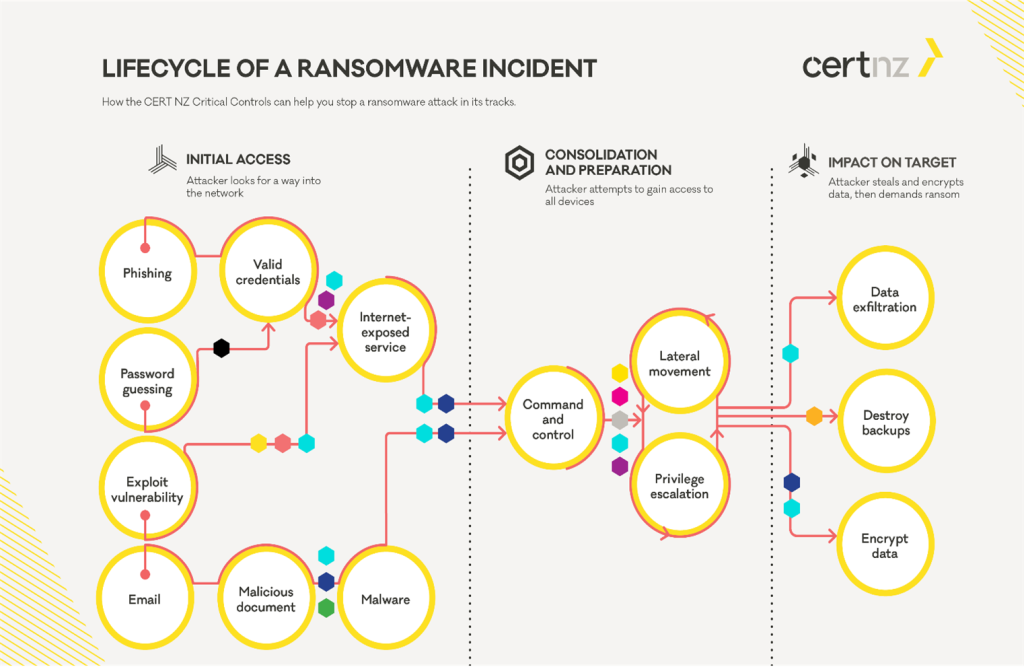
\includegraphics[scale=0.55]{certnz_aa23-165a.png}
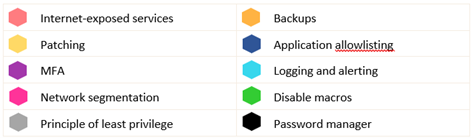
\includegraphics[scale=0.6]{certnz_aa23-165b.png}
\caption{Ransomware Layered Mitigations \autocite{Certnz:2021}}
\end{figure}

\pagebreak

%\subsection{Analysis of the impact and consequences of these incidents}
\subsection{Proposed solutions to improving our cyber-security measures}

As Security Joes is a security system vendor, the report itself lists a number of ways that the attack could be detected. In
the first instance, we should be talking to our XDR vendor to ensure we have the functionality to automate these steps.  At
the very least we need to be able to perform ad-hoc scans across our infrastructure and windows systems to flag the following:

\begin{enumerate}
\item Build a custom scan across our real estate and construct a database of trusted PE files that have a default RWX section.
\item Monitor for the launching of GNU utilities, as these were exploited by the attack.
\item Ensure our network scanning is looking for network connections to non-standard ports.
\item Investigate how to detect the loading of NTDLL.DLL without false positives.
\end{enumerate}


\subsection{Recommendations}

Our organisation is committed to the continued review of new attacks and actively researches the possible impact of reported attacks.
This active engagement with the cybersecurity community and our vendors allows us to adapt quickly to changes in the threat landscape.

For this case study, we recommend the following actions under each of the NIST CSF functions:

\begin{itemize}
\item \textbf{Identify}: Ensure all systems are patched for the CVEs identified and engage with our XDR vendor to respond to this new threat.
\item \textbf{Protect}: Review XDR solutions are monitoring systems to detect encryption and exfiltration attempts.
\item \textbf{Detect}: Develop a Mockingjay red-team exercise against our XDR; work with our vendor to track and monitor the loading of specific
  DLLs, including NTDLL.dll, by non-legitimate processes.
\item \textbf{Respond}: Ensure that our organisation can report to all relevant authorities and abide by our legal
  responsibilities for disclosures.
\item \textbf{Recover}: Follow up with internal teams to show recovery procedures from backup are up to date and ensure backups
  are held for all systems and are immutable. 
\end{itemize}
